%%%============================================================================
%     Run pdflatex  on this file in your command prompt of LaTeX environment of
%     your choice, if you want to typeset this document. 
%     The Document is Copyright 2012 by Thøger Rivera-Thorsen. You are free to
%     use it as you please under the terms of the GNU Free Document License
%     (FDL) as found on http://www.gnu.org/copyleft/fdl.html .
%%%============================================================================
\documentclass[a4paper, 11pt]{article} % Or book, memoir, letter, report, ...
% Hyphenation, date formats etc. - the last listed language is set by default:
\usepackage[swedish, english]{babel}
% Extended math support:
\usepackage{amsmath}
% Unicode gives better support for non-english characters etc.:
\usepackage[utf8]{inputenc}
% Correct hyphenation patterns + prettier fonts:
\usepackage[T1]{fontenc}
% Use graphics/images that are not just .eps format:
\usepackage[pdftex]{graphicx}
% Add capability of hyperlinking
\usepackage[breaklinks, pdftex]{hyperref}
% Try commenting out the following and see what happens:
\hypersetup{colorlinks=true}


\title{An example \LaTeX{} document}
\author{Thøger Rivera-Thorsen}
\date{\today}


\begin{document}

\maketitle

\begin{abstract}
This is a small and simple document written in \LaTeX{} to show the 
capabilities and workings of the software package. The source code of this
document contains many tips and tricks and explanations that are not visible in
the final document.

\textsc{Use the Source, Luke!}
\end{abstract}

\tableofcontents
\newpage
\listoffigures
\listoftables
\newpage


\section{The first section}
% Try to write \section*{title} instead - what happens?

This section is about the basic work with text in \LaTeX{}.  It is a little
different than one would think.  


%   \subsection{Demonstrate dynamic referencing}
%   
%   This little subsection can be commented out to show how references in later
%   sections update when their numbering changes. NB: you may need to run
%   \texttt{(pdf-)latex} twice before it updates correctly.


\subsection{Where's my line break?! \label{sec:linbre}}

For instance, no matter how many spaces I            add, it will not be 
visible in the document. 
Second, even if I add a line break, it is not respected! and if I add an empty
line, it will not be an empty line, but simply a new paragraph!

This is different than you're used to, but it means that a paragraph, which is
a ``structural unit of content'' in your text, also will be clearly visible as
a block of text in the source code, as can be seen by reading the source text
itself.

% Notice above that instead of normal quotation marks, I use the ``backtick''
% ` character for opening quotes and an apostrophe for a closing quote.

This way, one is brought to think about paragraphs, chapters, sections,
subsections etc. rather than headlines, bold or italic font, page breaks and
whatnot. All this is automatically taken care of\footnote{This also has the
very nice side effect that footnotes, chapter numbering etc. is taken care of
automatically - no sweat!} by the typesetting engine.


\subsection{Another subsection}

As one can see by studying the source code, numbering of sections, subsections
etc. is also taken care of automatically. Also, I can refer to a section (or
other structural element) by a \emph{label} rather than its number, for
instance to section ~\ref{sec:linbre}. Try to insert an extra subsection before
it and see what happens!

\subsection{A few more things}

The idea of thinking structure and content rather than looks can go against some
pretty set habits sometimes. Like the one of using \textit{italics} to emphasise
something in the text \emph{when we want something to
stand out}. The \texttt{emph} command does this intellegently,
writes the word in italics if the rest of the text is upright and vice versa.


\textit{
The idea of thinking structure and content rather than looks can go against some
pretty set habits sometimes. Like the one of using \textit{italics} to emphasise
something in the text \emph{when we want something to
stand out}. The \texttt{emph} command does this intellegently,
writes the word in italics if the rest of the text is upright and vice versa.}

\subsection{Lists}

There are different kinds of lists: numbered, bullet- and descriptive
lists, in the shape of the \texttt{itemize}, \texttt{enumerate} and
\texttt{description} environments. Here's how they work:


\subsubsection{The \texttt{enumerate} environment}

\begin{enumerate}
	\item Item 1
	\item Item 2
	\item \begin{enumerate}
			\item They can
			\item also be 
			\item nested!
	       \end{enumerate}
	\item And so on.
	\item \ldots
\end{enumerate}


\subsubsection{The \texttt{itemize} environment}

\begin{itemize}
	\item Item 1
	\item Item 2
	\item \begin{enumerate}
			\item They can
			\item also be 
			\item nested!
		\end{enumerate}
	\item And so on.
	\item \ldots
\end{itemize}


\subsubsection{The \texttt{description} environment}

\begin{description}
	\item[First item] This environment is more suitable for longer pieces
		of text, as can be seen here where I fill in a lot of text just
		so you can see that it looks better with more text, not just a
		little text. Don't you think that looks better?
	\item[Second Item] This environment is more suitable for longer pieces
		of text, as can be seen here where I fill in a lot of text just
		so you can see that it looks better with more text, not just a
		little text. Don't you think that looks better?
	\item[Third item] This environment is more suitable for longer pieces
		of text, as can be seen here where I fill in a lot of text just
		so you can see that it looks better with more text, not just a
		little text. Don't you think that looks better?
	\item[Third item] \ldots \ldots and on and on.
\end{description}


\section{Other elements: math, images, tables etc.}

This section will show how to do fancy stuff like math, tables and figures with
images in them.


\subsection{Mathematical notation}

The typesetting of mathematical expressions is where \LaTeX{} really shines. Its
text input ``language'' is logically built, and the output looks far better
than almost any other program out there. Maths can be shown in three different
ways: either inline in the text, in which case the math code is surrounded by
\texttt{\$[math expression here]\$} in the source text. That way, a simple
equation like e.g. $\Delta E_{kin}=\frac{1}{2}m \Delta v^2$ can be easily
integrated into the text. 

Or it can be shown as a single equation for itself. This can be done either
enclosed in double \texttt{\$\$}'s:

$$\Delta E_{kin}=\frac{1}{2}m\Delta v^2$$

or in the \texttt{equation} environment, in which case it will be automatically
numbered: 

\begin{equation}
	\Delta E_{kin}=\frac{1}{2}m\Delta v^2
	\label{eqn:ekin}
\end{equation}

Finally theres the case where we have several equations or a long derivation
that we want lined up nicely with the $=$ signs above each other. To this, we
use the \texttt{align} environment: \footnote{There is also an
\texttt{eqnarray} environment that does the same and that one will
see in many manuals - it is an older environment and is considered obsolete
in favor of \texttt{align}.}

\begin{align}
       A &= B \\
       C &= D \\
       E \neq F &= G
	\label{eqn:aligndemo}
\end{align}


\subsection{Floats: figures and tables}
One thing that can be very confusing to a beginner is the way \LaTeX{} handles
figures and tables. They are treated as \emph{floating objects}, which means
that they do not appear in the text exactly where they are put by the author. 

Rather, \LaTeX{} tries to fit them in where they fit best in the document. This
means that if you have many tables and figures, changing a few words can change
the layout of the floats and hence the entire document significantly. This is on
purpose and is meant to be that way. 


\subsubsection{Figure}

Here is how one can insert a figure (it is inserted here in the source text):
\begin{figure}[h]
	\begin{center}
		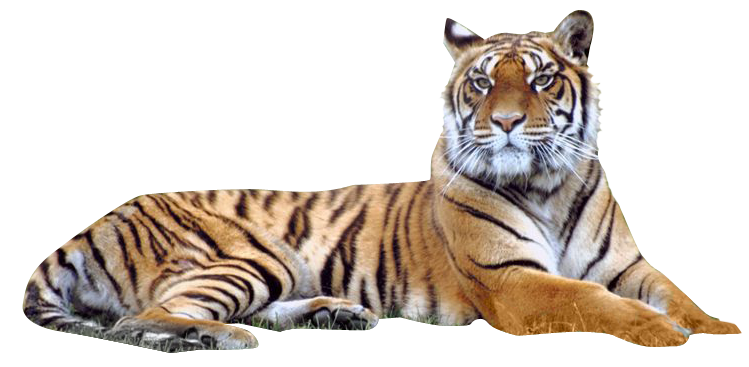
\includegraphics[width=.75\textwidth]{./tiger.png}
	\end{center}
	\caption[Badly photoshopped tiger]{This is a very, very dangerous Tiger! It is also offendingly
	bad photoshopping.}
	\label{fig:tiger}
\end{figure}

The figure is automatically numbered like anything else, and can be referred to
if one remembered to give it a label. Try to remove the surrounding
\texttt{figure} environment and maybe also the \texttt{center} environment and
see what difference it makes.


\subsubsection{Tables}
Here is where the table is inserted in the source text:
\begin{table}
	\centering
	\begin{tabular}{|l|rrr|}
		\hline
		\textbf{My table} & Thing I & Thing II & Thing III \\
		\hline
		\hline
		Param I           & 1.1     & 2.2      & 3.3       \\
		Param II          & 4.4     & 5.5      & 6.6       \\
		Param III         & 7.7     & 8.8      & 9.9       \\
		\hline

	\end{tabular}
	\caption[Tabular/table]{This is a tabular inside a table. Tabular is to table more or
	less what image/graphics is to figure. }
	\label{tab:tabul}
\end{table}


\section{Further reading}
Needless to say, I have only just scratched the surface here. \LaTeX{} is a huge
piece of software with a huge set of features and a mindbogglingly vast set of
packages that can provide even more features. 
There is lots of litterature about \LaTeX{}, I will recommend these two works as
great for both the beginner and the more seasoned \TeX'er.

\begin{enumerate}
	\item The first one is ``The not so short introduction to
		\LaTeXe{}'' Writen by Tobias Oetiker. You can
		\href{http://tobi.oetiker.ch/lshort/lshort.pdf}{download the
			\textsc{pdf} here}.
		I recommend printing it; it is short and very good as a
		reference.
	\item The second one is from WikiBooks and is simply called
		'\LaTeX{}'; it can be
		\href{http://en.wikibooks.org/wiki/LaTeX/}{found online here}.
		It comes in both a printable \textsc{pdf} version and an online
		version, but the online \textsc{htmL} version is much, much 
		nicer and easier to search. I recommend you bookmark it or
		include the keyword ``wikibooks'' in your search engine text 
		field next time you search for \LaTeX{} help.
		
\end{enumerate}

\end{document}
